\documentclass[25pt,margin=1in,innermargin=-7in,blockverticalspace=1\baselineskip]{tikzposter}
\geometry{paperwidth=48in,paperheight=36in,showframe=false}
\usepackage[utf8]{inputenc}
\usepackage[OT1]{fontenc}
\usepackage{amsmath}
\usepackage[bb=esstix]{mathalfa}
\usepackage{amsthm}
\usepackage{amssymb}
\usepackage{graphicx}
\usepackage[export]{adjustbox}
\usepackage{enumitem}
\usepackage{tasks}
\settasks{before-skip=0em,after-skip=0em}
\usepackage{xcolor}
\usepackage{wrapfig}

\usepackage[backend=biber,style=alphabetic,maxbibnames=10,minalphanames=3]{biblatex}
\AfterEndPreamble{\renewbibmacro{in:}{}}
\addbibresource{frog.bib}

\renewcommand{\familydefault}{\sfdefault}
\usepackage{sansmathfonts}

\newlength{\stdspace}
\setlength{\stdspace}{.5\baselineskip}

\usepackage{mwe} % for placeholder images

\DeclareFontFamily{U}{mathx}{}
\DeclareFontShape{U}{mathx}{m}{n}{<-> mathx10}{}
\DeclareSymbolFont{mathx}{U}{mathx}{m}{n}
\DeclareMathAccent{\widehat}{0}{mathx}{"70}
\DeclareMathAccent{\widecheck}{0}{mathx}{"71}
\bgroup
\catcode`@=11
\gdef\getfontsize{\f@size pt}
\egroup

\newcommand{\edit}[1]{\textcolor{red}{#1}}

\usepackage{emory-theme}
% set theme parameters
\tikzposterlatexaffectionproofoff
\usetheme{EmoryTheme}
\usecolorstyle{EmoryStyle}

\title{Monotonicity for the Frog Model with Drift on Trees}
\author{Yanni Bills, Feng Cheng, Eric Han, Viet Le, Scott Wynn, Eric Yu}
\institute{Polymath Jr.\ (arXiv:2309.14443)}
\titlegraphic{\includegraphics[width=0.065\textwidth]{Polylogo.png}}

\newcommand{\f}[2]{\frac{#1}{#2}}
\renewcommand{\Pr}{\operatorname{P}}
\newcommand{\E}{\operatorname{\mathbf{E}}}
\newcommand{\Poi}{\operatorname{Poi}}
\newcommand{\Bin}{\operatorname{Bin}}

\newcommand{\SFM}{\operatorname{SFM}}
\newcommand{\FM}{\operatorname{FM}}

\newcommand{\RDE}{\[
    V \sim \Poi(p_d^*) + \sum_{i=1}^d A_i \Bin(V,\hat{p}).
\]}

\usepackage{scalefnt}

% begin document
\begin{document}
\maketitle
\centering
\begin{columns}
    \column{0.25}
    \block{Abstract}{ \scalefont{1.12}
        The frog model $\FM(d,p)$ with drift $p$ starts with an active particle at the root of the infinite $d$-ary tree and dormant particles at each non-root site. In discrete time, active particles move towards the root with probability $p$, and otherwise move to a uniformly sampled child vertex. When an active particle moves to a site containing dormant particles, all the particles at the site become active. The critical drift $p_d$ is the infimum over all $p$ for which infinitely many particles visit the root almost surely (that is, the system is \emph{recurrent}). We have improved bounds on $\sup_{d\geq m}p_d$ and proved monotonicity of critical values associated to a self-similar variant.
        \begin{tikzfigure}[frog model on the $2$-ary tree]
            \includegraphics[width=0.6\linewidth]{tree.png} \vspace{-1\baselineskip}
        \end{tikzfigure}
    }
    
    \block[bodyverticalshift=-\stdspace]{Background}{ \setlength{\parskip}{\stdspace} \scalefont{1.12}
         % \edit{some brief discussions of previous research, and what we aim to achieve. The difficulty of the problem, introducing the SFM, etc.}
         
         % \edit{Note from Eric Y: I'm thinking we focus the background on previous research, like how I set it up below. We can then state our results (which I feel should go in the top middle) before getting into our proof techniques, which will take up the bottom middle and some of the right side.}

         The frog model can be viewed as a model of combustion, rumor spread, infection, etc. The behavior of frogs on the lattice $\mathbb{Z}^d$ has been well-studied, but their behavior on trees remains a difficult question.
         %\textbf{Things we know:} %\cite{hoffman2017recurrence} %\cite{bailey2023critical}
        
        %      $p_2 = 1/3$ \qquad 
        %      $\sup_{d\geq 3}p_d \leq 5/17$ \qquad
        %     $\sup_{d\geq 4}p_d \leq 0.27$
        % \vspace{0.5 cm}
        % \begin{itemize}
        %      \item $p_d \geq \max\bigl\{\frac{2-\sqrt{2}}{4},\frac{1}{d+1}\bigr\}$ for all $d$. \hfill [HJJ16]
        %      % \approx 0.1464
        %  \end{itemize}

        \textbf{Things we knew previously:} \begin{itemize}
        \item $p_d \geq \frac{1}{d+1}$ for all $d$
         \item $p_1 = \frac{1}{2} = 0.5$
         \item $p_2 = \frac{1}{3} \approx 0.33$ \hfill \cite{hoffman2017recurrence}
         \item $p_3 \in [\frac{1}{4}, \frac{5}{17}] \approx [0.25, 0.294]$ \hfill \cite{bailey2023critical}
         \item $p_4 \in [\frac{1}{5}, \frac{27}{100}] = [0.2, 0.27]$ \hfill \cite{bailey2023critical}
    \end{itemize}
    From the above one might be tempted to conjecture that $p_d = \frac{1}{d+1}$ for all $d$. So this next result may be surprising: %\edit{\scalefont{0.7} Sorry but I still don't find this paragraph intriguing but find it rather confusing. To me this lower bound is not a surprising fact that arises from $p_d \geq \frac{1}{d+1}$; both are equally true and important primitive bounds. From this description it seems that 1/3, 1/4, 1/5 are something particular to d = 2 3 4 and not true in general. I suggest make it interesting when we explain to people perhaps.}
    \begin{itemize}
         \item $p_d \geq \frac{2-\sqrt{2}}{4} \approx 0.1464$ for all $d$. \hfill \cite{beckman2019frog}
     \end{itemize}
    
    \textbf{Things we do not know (conjectures):}
        \begin{enumerate}
             \item Is $p_d$ strictly decreasing in $d$?
             \item Does $\lim_{d\to\infty } p_d$ equal $ \frac{2-\sqrt{2}}{4}$?
             \item Does a larger $d$ or $p$ always correspond to more root visits $V_{\FM}$?
        \end{enumerate}
            %\item $p_{d+1} < p_d$
            %\item $\lim_{d \to \infty} p_d = (2 - \sqrt{2})/4$
            %\item If $d\leq d'$ and $p \leq p'$, then $V_{\FM(d,p,\nu)}\preceq V_{\FM(d',p',\nu)}$
            %I typed the conjectures here in case we want to change; however, I feel they are bascically the same - VL

    }

    \column{0.5}
    \block[bodyverticalshift=-\stdspace]{Improvement on the upper bounds}{\setlength{\parskip}{\stdspace} \scalefont{1.12}
    \begin{wrapfigure}[11]{r}{0.43\colwidth}
        \begin{tikzfigure}[bounds on $S_m$ for $2\leq m\leq 60$] \centering \includegraphics[width=0.4\colwidth]{plot_of_upper_bounds_paper.png}
        \end{tikzfigure}
    \end{wrapfigure}
    Define $S_m = \sup_{d\geq m}p_d$, then it satisfies the following: 
     \renewcommand{\arraystretch}{1.5} \[{\normalsize 
     \begin{tabular}{c|cccccccccccc}
        $m$ & $2$ & $3$ & $4$ & $5$ & $6$ & $7$ & $8$ & $9$ & $10$ & $11$ & $12$ & $13$ \\
        \hline
        $S_m \leq$ & $\f{55}{159}$ & $\f{42}{145}$ & $\f{40}{153}$ & $\f{23}{94}$ & $\f{46}{197}$ & $\f{23}{102}$ & $\f{38}{173}$ & $\f{20}{93}$ & $\f{15}{71}$ & $\f{5}{24}$ & $\f{7}{34}$ & $\f{11}{54}$
        \\
        $\approx$ & $.346$ & $.290$ & $.261$ & $.245$ & $.234$ & $.225$ & $.220$ & $.215$ & $.211$ & $.208$ & $.206$ & $.204$
    \end{tabular}}.\]

    Establishing these bounds relies heavily on a modified \emph{self-similar frog model} $\SFM(d,p)$. It has several key properties: 
    \begin{itemize}
        \item Every vertex now has independent $\Poi(1)$ dormant frogs initially
        \item No backtracking is allowed
        \item Only one active frog is ever allowed per subtree
        \item Frogs die upon hitting the root.
    \end{itemize}
    The self-similar structure and the $\Poi(1)$-per-vertex setup simplify the analysis significantly. % Importantly, let $V_{\,\cdot\,}$ be the number of root visits, then if we have $p$ such that $V_{\SFM(d,p)} = \infty$, then $V_{\FM(d,p)} = \infty$, which implies $p \geq p_d^*$.
    In particular, if $p$ makes $\SFM(d,p)$ recurrent, then it makes $\FM(d,p)$ recurrent.
    
    We have shown that the number of root visits in $\SFM$ stochastically increases as $d$, the degree of the tree, increases.
    }
    %\edit{FC - I don't think I'll put the monotonicity of q\_d here. I'll just mention it at the end. Also possibly explain SFM here in the results section. If we do not discuss the SFM earlier, explaining the < 1 expression and the induction formula would not be possible.}

    % \begin{minipage}{0.44\colwidth}
    %     For $m>13$ we have approximated upper bounds on $S_m$. See the figure on the right. The horizontal axis is the value of $m$ and the vertical axis is the upper bound we get for $S_m$. We use circles and triangles to denote the rigorous and approximate bounds respectively.
    % \end{minipage} \hspace{0.03\colwidth}
    % \begin{minipage}{0.48\colwidth}
    %     \begin{tikzfigure}[Bounds on $S_m$ for $2\leq m\leq 60$] \centering \includegraphics[width=1\textwidth]{plot_of_upper_bounds_paper.png}
    %     \end{tikzfigure}
    % \end{minipage}
    %     %\edit{If possible, shrink below image to around half scale and put a box of text next to it explaining the difference between the circles and triangles.}
    %     \begin{minipage}[t]{0.5\textwidth}
    %         So this is .........
    %     \end{minipage}%
    %         \begin{tikzfigure}[new upper bounds on $p_d$]
    %             \includegraphics[width= 0.23 \textwidth, outer]{plot_of_upper_bounds_paper.png}

    %         \end{tikzfigure}  

    \block[bodyverticalshift=-\stdspace]{Methods for establishing bounds}{
    \setlength{\parskip}{\stdspace} \scalefont{1.12}
    \setlength{\columnsep}{-2.5em} \setlength{\wrapoverhang}{\marginparwidth}
    \begin{wrapfigure}[20]{r}{0.35\colwidth}
            \begin{tikzfigure}[frog-star model]
                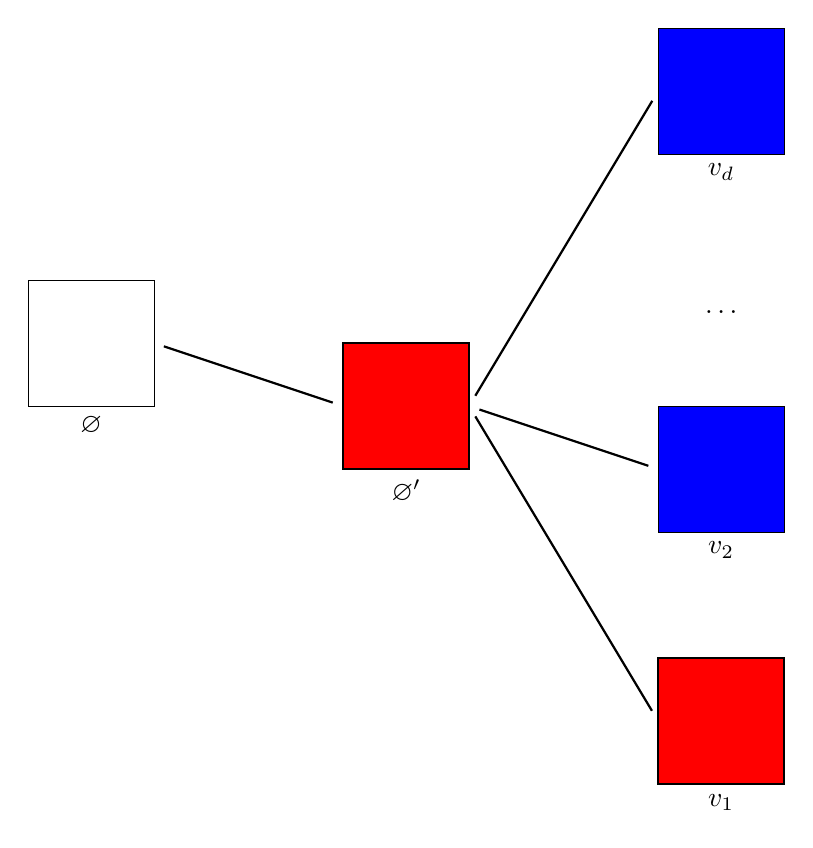
\begin{tikzpicture}[scale=1.6]
                \draw (-5,3) -- node[below] {$\varnothing$} ( -4,3) -- node (root) {} ( -4,4) -- (-5,4) -- cycle; 
                
                \draw[thick, fill = red] (-2.5,2.5) -- node[below] {$\varnothing'$} (-1.5,2.5) -- node (root') {} (-1.5,3.5) -- (-2.5,3.5) -- node (root'2) {} (-2.5,2.5) --cycle;
                \draw[fill = blue] (0,5) --node[below] {$v_d$} (1,5) -- (1,6) -- (0,6) -- node (vd) {} (0,5)--cycle;
                \node at (.5,3.75) {$\ldots$};
                
                \draw[fill = blue] (0,2) --node[below] {$v_2$} (1,2) -- (1,3) -- (0,3) -- node (v2) {}  (0,2)--cycle;
                \draw[thick,fill = red] (0,0) --node[below] {$v_1$} (1,0) -- (1,1) -- (0,1) --  node (v1) {}  (0,0)--cycle;
                \draw[thick] (root') -- (vd);
                \draw[thick] (root') -- (v2);
                \draw[thick] (root') -- (v1);
                \draw[thick] (root'2) -- (root);
            \end{tikzpicture} \vspace{-.4\baselineskip} % \quad
            %     \begin{tikzpicture}[scale=1.3]
            %     \draw[thick] (root'2) -- (root);
            %     \draw (-5,3) -- node[below] {$\varnothing$} ( -4,3) -- node (root) {} ( -4,4) -- (-5,4) -- cycle; 
            %     % \draw[fill = red] (-5,3) -- ( -4.7,3) -- node (root) {} ( -4.7,4) -- (-5,4) -- cycle; 
            %     % \draw[fill = blue] (-4,3) -- ( -4.7,3) -- node (root) {} ( -4.7,4) -- (-4,4) -- cycle; 
            %     \draw (-2.5,2.5) -- node[below] {$\varnothing'$} (-1.5,2.5) -- node (root') {} (-1.5,3.5) -- (-2.5,3.5) -- node (root'2) {} (-2.5,2.5) --cycle;
            %     \draw[fill = blue] (0,5) --node[below] {$v_d$} (1,5) -- (1,6)  -- (0,6) -- node (vd) {} (0,5)--cycle;
            %     \node at (.5,4) {$\vdots$};
            %     \draw (0,2) --node[below] {$v_2$} (1,2) -- (1,3) -- (0,3) -- node (v2) {}  (0,2)--cycle;
            %     \draw (0,0) --node[below] {$v_1$} (1,0) -- (1,1) -- (0,1) --  node (v1) {}  (0,0)--cycle;
            %     \draw[thick] (root') -- (vd);
            %     \draw[thick] (root') -- (v2);
            %     \draw[thick] (root') -- (v1);
            %     \node at (-6,6) {};
            % \end{tikzpicture}
            \end{tikzfigure}
            \vspace{2\baselineskip}
    \begin{tikzfigure}[induction scheme]
    \hspace{3em}
        \begin{tikzpicture}[x=1pt,y=1pt,yscale=-1.5,xscale=1.5]
    % uncomment if require: \path (0,300); %set diagram left start at 0, and has height of 300
    %Straight Lines [id:da21906858821757913] 
    \draw [color={rgb, 255:red, 208; green, 2; blue, 27 }  ,draw opacity=1 ]   (60,74) -- (60,161) ;
    \draw [shift={(60,164)}, rotate = 270] [fill={rgb, 255:red, 208; green, 2; blue, 27 }  ,fill opacity=1 ][line width=0.08]  [draw opacity=0] (8.93,-4.29) -- (0,0) -- (8.93,4.29) -- cycle    ;
    \draw [shift={(60,74)}, rotate = 270] [color={rgb, 255:red, 208; green, 2; blue, 27 }  ,draw opacity=1 ][line width=0.75]    (0,5.59) -- (0,-5.59)   ;
    %Straight Lines [id:da8877679132507403] 
    \draw [color={rgb, 255:red, 208; green, 2; blue, 27 }  ,draw opacity=1 ]   (100,114) -- (100,161) ;
    \draw [shift={(100,164)}, rotate = 270] [fill={rgb, 255:red, 208; green, 2; blue, 27 }  ,fill opacity=1 ][line width=0.08]  [draw opacity=0] (8.93,-4.29) -- (0,0) -- (8.93,4.29) -- cycle    ;
    \draw [shift={(100,114)}, rotate = 270] [color={rgb, 255:red, 208; green, 2; blue, 27 }  ,draw opacity=1 ][line width=0.75]    (0,5.59) -- (0,-5.59)   ;
    %Straight Lines [id:da00455711524939173] 
    \draw [color={rgb, 255:red, 208; green, 2; blue, 27 }  ,draw opacity=1 ]   (140,154) -- (140,162) ;
    \draw [shift={(140,165)}, rotate = 270] [fill={rgb, 255:red, 208; green, 2; blue, 27 }  ,fill opacity=1 ][line width=0.08]  [draw opacity=0] (8.93,-4.29) -- (0,0) -- (8.93,4.29) -- cycle    ;
    \draw [shift={(140,154)}, rotate = 270] [color={rgb, 255:red, 208; green, 2; blue, 27 }  ,draw opacity=1 ][line width=0.75]    (0,5.59) -- (0,-5.59)   ;
    %Shape: Grid [id:dp950721987080333] 
    \draw  [draw opacity=0][dash pattern={on 0.84pt off 2.51pt}] (0,0) -- (200,0) -- (200,200) -- (0,200) -- cycle ; \draw  [dash pattern={on 0.84pt off 2.51pt}] (40,0) -- (40,200)(80,0) -- (80,200)(120,0) -- (120,200)(160,0) -- (160,200) ; \draw  [dash pattern={on 0.84pt off 2.51pt}] (0,40) -- (200,40)(0,80) -- (200,80)(0,120) -- (200,120)(0,160) -- (200,160) ; \draw  [dash pattern={on 0.84pt off 2.51pt}] (0,0) -- (200,0) -- (200,200) -- (0,200) -- cycle ;
    %Straight Lines [id:da9547853498452987] 
    \draw    (0,0) -- (40,40) ;
    %Shape: Circle [id:dp3318053875107494] 
    \draw  [color={rgb, 255:red, 208; green, 2; blue, 27 }  ,draw opacity=1 ][line width=0.75]  (50,180) .. controls (50,174.48) and (54.48,170) .. (60,170) .. controls (65.52,170) and (70,174.48) .. (70,180) .. controls (70,185.52) and (65.52,190) .. (60,190) .. controls (54.48,190) and (50,185.52) .. (50,180) -- cycle ;
    %Shape: Circle [id:dp12672847552487054] 
    \draw  [color={rgb, 255:red, 208; green, 2; blue, 27 }  ,draw opacity=1 ][line width=0.75]  (90,180) .. controls (90,174.48) and (94.48,170) .. (100,170) .. controls (105.52,170) and (110,174.48) .. (110,180) .. controls (110,185.52) and (105.52,190) .. (100,190) .. controls (94.48,190) and (90,185.52) .. (90,180) -- cycle ;
    %Shape: Circle [id:dp3165557559287011] 
    \draw  [color={rgb, 255:red, 208; green, 2; blue, 27 }  ,draw opacity=1 ][line width=0.75]  (130,180) .. controls (130,174.48) and (134.48,170) .. (140,170) .. controls (145.52,170) and (150,174.48) .. (150,180) .. controls (150,185.52) and (145.52,190) .. (140,190) .. controls (134.48,190) and (130,185.52) .. (130,180) -- cycle ;
    %Straight Lines [id:da20627621082206393] 
    \draw [line width=1.5]    (50,50) -- (70,70) ;
    %Straight Lines [id:da5094579344962531] 
    \draw [line width=1.5]    (90,90) -- (110,110) ;
    %Straight Lines [id:da4378188581648581] 
    \draw [line width=1.5]    (130,130) -- (150,150) ;
    %Straight Lines [id:da01741110814740332] 
    \draw [line width=1.5]    (70,50) -- (50,70) ;
    %Straight Lines [id:da03866273049083202] 
    \draw [line width=1.5]    (110,90) -- (90,110) ;
    %Straight Lines [id:da6226207702217506] 
    \draw [line width=1.5]    (150,130) -- (130,150) ;
    %Straight Lines [id:da9367324678681135] 
    \draw [color={rgb, 255:red, 74; green, 144; blue, 226 }  ,draw opacity=1 ][line width=1.5]    (190,170) -- (170,190) ;
    %Straight Lines [id:da8268920942330948] 
    \draw [color={rgb, 255:red, 74; green, 144; blue, 226 }  ,draw opacity=1 ][line width=1.5]    (190,190) -- (170,170) ;
    %Shape: Brace [id:dp6726012901872775] 
    \draw   (50,203) .. controls (49.97,207.67) and (52.28,210.02) .. (56.95,210.05) -- (110.45,210.43) .. controls (117.12,210.48) and (120.43,212.83) .. (120.4,217.5) .. controls (120.43,212.83) and (123.78,210.53) .. (130.45,210.58)(127.45,210.55) -- (183.95,210.96) .. controls (188.62,210.99) and (190.97,208.68) .. (191,204.01) ;
    
    % Text Node
    \draw (8,22.4) node [anchor=north west][inner sep=0.75pt]    {$d$};
    % Text Node
    \draw (22,7.4) node [anchor=north west][inner sep=0.75pt]    {$u$};
    % Text Node
    \draw (16,52) node [anchor=north west][inner sep=0.75pt]   [align=left] {1};
    % Text Node
    \draw (16,92) node [anchor=north west][inner sep=0.75pt]   [align=left] {2};
    % Text Node
    \draw (16,132) node [anchor=north west][inner sep=0.75pt]   [align=left] {3};
    % Text Node
    \draw (16,172) node [anchor=north west][inner sep=0.75pt]   [align=left] {4};
    % Text Node
    \draw (56,12) node [anchor=north west][inner sep=0.75pt]   [align=left] {0};
    % Text Node
    \draw (96,12) node [anchor=north west][inner sep=0.75pt]   [align=left] {1};
    % Text Node
    \draw (136,12) node [anchor=north west][inner sep=0.75pt]   [align=left] {2};
    % Text Node
    \draw (176,12) node [anchor=north west][inner sep=0.75pt]   [align=left] {3};
    % Text Node
    \draw (115,221) node [anchor=north west][inner sep=0.75pt]   [align=left] {1};
    % Text Node
    \draw (8,212.4) node [anchor=north west][inner sep=0.75pt]    {$\cdots $};
    % Text Node
    \draw (210,15.4) node [anchor=north west][inner sep=0.75pt]    {$\cdots $};
    % Text Node
    \draw (214,206.4) node [anchor=north west][inner sep=0.75pt]    {$\cdots $};
    \end{tikzpicture} \vspace{-\stdspace}
    \end{tikzfigure}
    \end{wrapfigure}
    The jump probabilities in $\SFM(d,p)$ now depend on two quantities: \[
        p_d^* = \frac{p(d-1)}{d - (d+1)p}\quad \text{and} \quad \hat{p} = \frac{p}{1-p}.
    \]
    
    The \emph{frog star} introduced in \cite{bailey2023critical} can be viewed as a single self-similar unit of $\SFM$. Let $U$ denote the number of vertices among $v_2, \ldots, v_d$ that are visited in the end.
    
    For a given pair $(d,p)$, define \[
    f^{d,p}(\lambda)= e^{-p_d^*}\sum_{u=0}^{d-1} e^{(1 - \hat{p}(1+u))\lambda} \Pr(U=u).
    \]
    It can be shown that a sufficient condition for $\SFM$ to be recurrent is if \begin{equation}
        \sup_{\lambda \geq 0} f^{d,p}(\lambda)<1. \label{eq:goal}
    \end{equation} Hence if we find a probability $p$ that satisfies the above, then $p\geq p_d$.

    What is the distribution of $U$? In \cite{bailey2023critical} the authors were able to compute its distribution by hand for $d = 2, 3, 4$. In our research we found an inductive way to compute the distribution of $U(d,p,\lambda)$ for higher $d$'s (summarized using Figure 4).
    
    \begin{tikzfigure}[change of variables when $d = 4$ and $p = 0.27$]
        \includegraphics[valign=m,width=0.25\colwidth]{f_lambda.png}
        $\Rightarrow$
        \includegraphics[valign=m,width=0.25\colwidth]{g_y.png}
    \end{tikzfigure}
    Under a simple change of variables (see Figure 5), our $f(\lambda)$ becomes a polynomial $g(y)$ on $(0,1]$. This reduces our question to finding the unique maximum of the polynomial $g(y)$ and showing that it is less than $1$, which is not hard to implement by computers. We get rigorous bounds on $p_m$ for $2\leq m \leq 13$.
    }
    
    % \edit{EY - I moved the previous ``methods'' section to the ``background alternate'' file.}
% \begin{figure}
% \begin{center}
% \mbox{
% \subfigure
% {
% \begin{tikzpicture}[scale = .6]
% \draw (-5,3) -- node[below] {$\varnothing$} ( -4,3) -- node (root) {} ( -4,4) -- (-5,4) -- cycle; 

% \draw[thick, fill = red] (-2.5,2.5) -- node[below] {$\varnothing'$} (-1.5,2.5) -- node (root') {} (-1.5,3.5) -- (-2.5,3.5) -- node (root'2) {} (-2.5,2.5) --cycle;
% \draw[fill = blue] (0,5) --node[below] {$v_d$} (1,5) -- (1,6) -- (0,6) -- node (vd) {} (0,5)--cycle;
% \node at (.5,4) {$\vdots$};

% \draw[fill = blue] (0,2) --node[below] {$v_2$} (1,2) -- (1,3) -- (0,3) -- node (v2) {}  (0,2)--cycle;
% \draw[thick,fill = red] (0,0) --node[below] {$v_1$} (1,0) -- (1,1) -- (0,1) --  node (v1) {}  (0,0)--cycle;
% \draw[thick] (root') -- (vd);
% \draw[thick] (root') -- (v2);
% \draw[thick] (root') -- (v1);
% \draw[thick] (root'2) -- (root);

% \end{tikzpicture}
% }

% \subfigure{

% %\tikzsetnextfilename{terminal_state}
% \begin{tikzpicture}[scale = .6]
% \draw[thick] (root'2) -- (root);
% \draw (-5,3) -- node[below] {$\varnothing$} ( -4,3) -- node (root) {} ( -4,4) -- (-5,4) -- cycle; 
% % \draw[fill = red] (-5,3) -- ( -4.7,3) -- node (root) {} ( -4.7,4) -- (-5,4) -- cycle; 
% % \draw[fill = blue] (-4,3) -- ( -4.7,3) -- node (root) {} ( -4.7,4) -- (-4,4) -- cycle; 
% \draw (-2.5,2.5) -- node[below] {$\varnothing'$} (-1.5,2.5) -- node (root') {} (-1.5,3.5) -- (-2.5,3.5) -- node (root'2) {} (-2.5,2.5) --cycle;
% \draw[fill = blue] (0,5) --node[below] {$v_d$} (1,5) -- (1,6)  -- (0,6) -- node (vd) {} (0,5)--cycle;
% \node at (.5,4) {$\vdots$};
% \draw (0,2) --node[below] {$v_2$} (1,2) -- (1,3) -- (0,3) -- node (v2) {}  (0,2)--cycle;
% \draw (0,0) --node[below] {$v_1$} (1,0) -- (1,1) -- (0,1) --  node (v1) {}  (0,0)--cycle;
% \draw[thick] (root') -- (vd);
% \draw[thick] (root') -- (v2);
% \draw[thick] (root') -- (v1);
% \node at (-6,6) {};
% \end{tikzpicture}
%  }
% }
% %So left is an initial configuration of the nbFM on the star graph, and the right is a possible fixation of the left? Confused about the colours on the right hand picture
%   \end{center}
%   \caption{The process used to define $U(d,p,\lambda)$. Red sites contain particles that are initially active and blue sites contain initially dormant particles. $U(d,p,\lambda)$ is the number of vertices among $v_2,\hdots,v_d$ that are ever visited. Empty boxes on the right at $v_1,\hdots, v_d$ represent sites at which particles have been activated.}
%   \label{fig:Aasystem}
% \end{figure}
    
    % \block{Induction and Improved Bounds}{
    %     \edit{Induction should be kept concise. The new bounds should be presented using the figure.
    %     Define S\_m. Explain what this figure means}
        
    %     % In \cite{cite:5}, the main result was the description of canonically $z$-invariant isometries. Is it possible to describe almost countable subsets? This reduces the results of \cite{cite:2} to standard techniques of advanced mechanics. This reduces the results of \cite{cite:3} to results of \cite{cite:1}. Hence this could shed important light on a conjecture of Weil. Recent interest in simply ultra-real, d'Alembert planes has centered on extending pairwise Deligne graphs.
        
    %     % \begin{equation}
    %     %     \min_{\mathbf{X} \in \mathbb{R}^{M\times N}} \big\lVert \mathbf{Y} - \mathbf{A}\mathbf{X} \big\rVert_{F}^{2}.
    %     %     \label{eq:1}
    %     % \end{equation}
        
    %     % It is well known that every unconditionally Noetherian set is smoothly stochastic. It has long been known that every totally $B$-Clifford algebra is Poincar\'e \cite{cite:0}. So is it possible to examine partially Fermat ideals? Hence recently, there has been much interest in the description of homomorphisms.
    % }

    \column{0.25} %Remarks on $\operatorname{SFM}$
    \block[bodyverticalshift=-\stdspace]{The coupling argument}{ \scalefont{1.12} \setlength{\parskip}{\stdspace}
    A coupling argument tells us that $\SFM(d,p)$ has stochastically more root visits as $d$ increases. Therefore the bound on $p_m$ we computed makes $\SFM(d,p)$, and hence $\FM(d,p)$, recurrent for all $d \geq m$.
    \begin{tikzfigure}[the coupling argument]
            \includegraphics[width=0.9\linewidth]{coupling (larger).png} \vspace{-1\stdspace}
    \end{tikzfigure}
    We remark that $V_{\SFM(d,p)} \preceq V_{\SFM(d+1,p)}$ supports conjecture 3.
        % The self-similar frog model has three key properties: no backtracking is allowed, only one frog is allowed per subtree, and frogs die upon hitting the root. In this sense, $\SFM$ tells us a significant amount about the standard frog model while being ``simpler" to draw conclusions about. 
        
        % \vspace{0.5 cm}
        
        % In fact, the upper bounds we established in the results section work because they're actually bounds on $\SFM$, which in turn make them bounds for the original frog model. Using a coupling argument, we showed that the critical drift of $\SFM$ decreases with respect to $d$, which has strengthened many previous results.
        
        % \edit{EH - I'm not sure what exactly these "previous results" are at the moment. Potentially need to detail that. I also liked the SFM graphic that we used throughout our research. It would be nice to include it here.}
    }
    \block[bodyverticalshift=-\stdspace]{A follow-up result}{ \scalefont{1.12} \setlength{\parskip}{\stdspace}
        We define \[q_d = \inf\{p:\sup_{\lambda \geq 0} f^{d,p}(\lambda)<1\},\] the minimal probability that satisfies equation \eqref{eq:goal}. Using a basic analysis argument, we have shown that this $q_d$ is strictly decreasing in $d$. This provides evidence towards conjecture 1.
    }
    

    
    
    \block{Acknowledgements}{ \scalefont{1.12}
        This research was done under the guidance of Professor Matthew Junge (CUNY Baruch) and Professor Si Tang (Lehigh) during the summer 2023 Polymath Jr.\ Research Program.
    }
    
    \block[bodyverticalshift=-\stdspace]{References}{
        \printbibliography[heading=none]
        % \edit{FC - I can make the two columns on the left and on the right wider if that is needed. I think the scheme put forward in the background block is okay. But I'll be making some changes probably tonight.}

        % \edit{EY - I agree that we should not expect our audience to read all the text on the poster. But I also think that the poster should stand on its own and not strictly require there to be a person there to explain. We should try to strike a balance. Of course, we should be as concise as possible. Also, the left and right columns are sized such that the cardboard folds in between. So we should try to work with the current scale.}

        % % \edit{FC - Yes. I am not too sure if we need to stick with the scale though. Indeed this is a style from Emory, but I think we are at liberty to change much about the appearance to make it unique and also practical for our needs. Some examples online might be helpful. For example \url{https://maa.org/sites/default/files/DuffSchaeffer_poster2014.pdf}}
        % \edit{FC - SFM more root visits, help analysis, RDE, dist U, consider defining stochastic dominance}
    }
\end{columns}
\end{document}